% Options for packages loaded elsewhere
\PassOptionsToPackage{unicode}{hyperref}
\PassOptionsToPackage{hyphens}{url}
%
\documentclass[
]{article}
\usepackage{amsmath,amssymb}
\usepackage{lmodern}
\usepackage{iftex}
\ifPDFTeX
  \usepackage[T1]{fontenc}
  \usepackage[utf8]{inputenc}
  \usepackage{textcomp} % provide euro and other symbols
\else % if luatex or xetex
  \usepackage{unicode-math}
  \defaultfontfeatures{Scale=MatchLowercase}
  \defaultfontfeatures[\rmfamily]{Ligatures=TeX,Scale=1}
\fi
% Use upquote if available, for straight quotes in verbatim environments
\IfFileExists{upquote.sty}{\usepackage{upquote}}{}
\IfFileExists{microtype.sty}{% use microtype if available
  \usepackage[]{microtype}
  \UseMicrotypeSet[protrusion]{basicmath} % disable protrusion for tt fonts
}{}
\makeatletter
\@ifundefined{KOMAClassName}{% if non-KOMA class
  \IfFileExists{parskip.sty}{%
    \usepackage{parskip}
  }{% else
    \setlength{\parindent}{0pt}
    \setlength{\parskip}{6pt plus 2pt minus 1pt}}
}{% if KOMA class
  \KOMAoptions{parskip=half}}
\makeatother
\usepackage{xcolor}
\usepackage[margin=1in]{geometry}
\usepackage{graphicx}
\makeatletter
\def\maxwidth{\ifdim\Gin@nat@width>\linewidth\linewidth\else\Gin@nat@width\fi}
\def\maxheight{\ifdim\Gin@nat@height>\textheight\textheight\else\Gin@nat@height\fi}
\makeatother
% Scale images if necessary, so that they will not overflow the page
% margins by default, and it is still possible to overwrite the defaults
% using explicit options in \includegraphics[width, height, ...]{}
\setkeys{Gin}{width=\maxwidth,height=\maxheight,keepaspectratio}
% Set default figure placement to htbp
\makeatletter
\def\fps@figure{htbp}
\makeatother
\setlength{\emergencystretch}{3em} % prevent overfull lines
\providecommand{\tightlist}{%
  \setlength{\itemsep}{0pt}\setlength{\parskip}{0pt}}
\setcounter{secnumdepth}{-\maxdimen} % remove section numbering
\pagenumbering{gobble}
\usepackage{booktabs}
\usepackage{longtable}
\usepackage{array}
\usepackage{multirow}
\usepackage{wrapfig}
\usepackage{float}
\usepackage{colortbl}
\usepackage{pdflscape}
\usepackage{tabu}
\usepackage{threeparttable}
\usepackage{threeparttablex}
\usepackage[normalem]{ulem}
\usepackage{makecell}
\usepackage{xcolor}
\ifLuaTeX
  \usepackage{selnolig}  % disable illegal ligatures
\fi
\IfFileExists{bookmark.sty}{\usepackage{bookmark}}{\usepackage{hyperref}}
\IfFileExists{xurl.sty}{\usepackage{xurl}}{} % add URL line breaks if available
\urlstyle{same} % disable monospaced font for URLs
\hypersetup{
  pdftitle={Multidimensional signals and analytic flexibility: Estimating degrees of freedom in human speech analyses},
  hidelinks,
  pdfcreator={LaTeX via pandoc}}

\title{Multidimensional signals and analytic flexibility:\\
Estimating degrees of freedom in human speech analyses}
\usepackage{etoolbox}
\makeatletter
\providecommand{\subtitle}[1]{% add subtitle to \maketitle
  \apptocmd{\@title}{\par {\large #1 \par}}{}{}
}
\makeatother
\subtitle{Supplementary materials}
\author{Initiating authors:\\
Stefano Coretta, Joseph V. Casillas, and Timo Roettger}
\date{2023-01-18}

\begin{document}
\maketitle

\begin{figure}
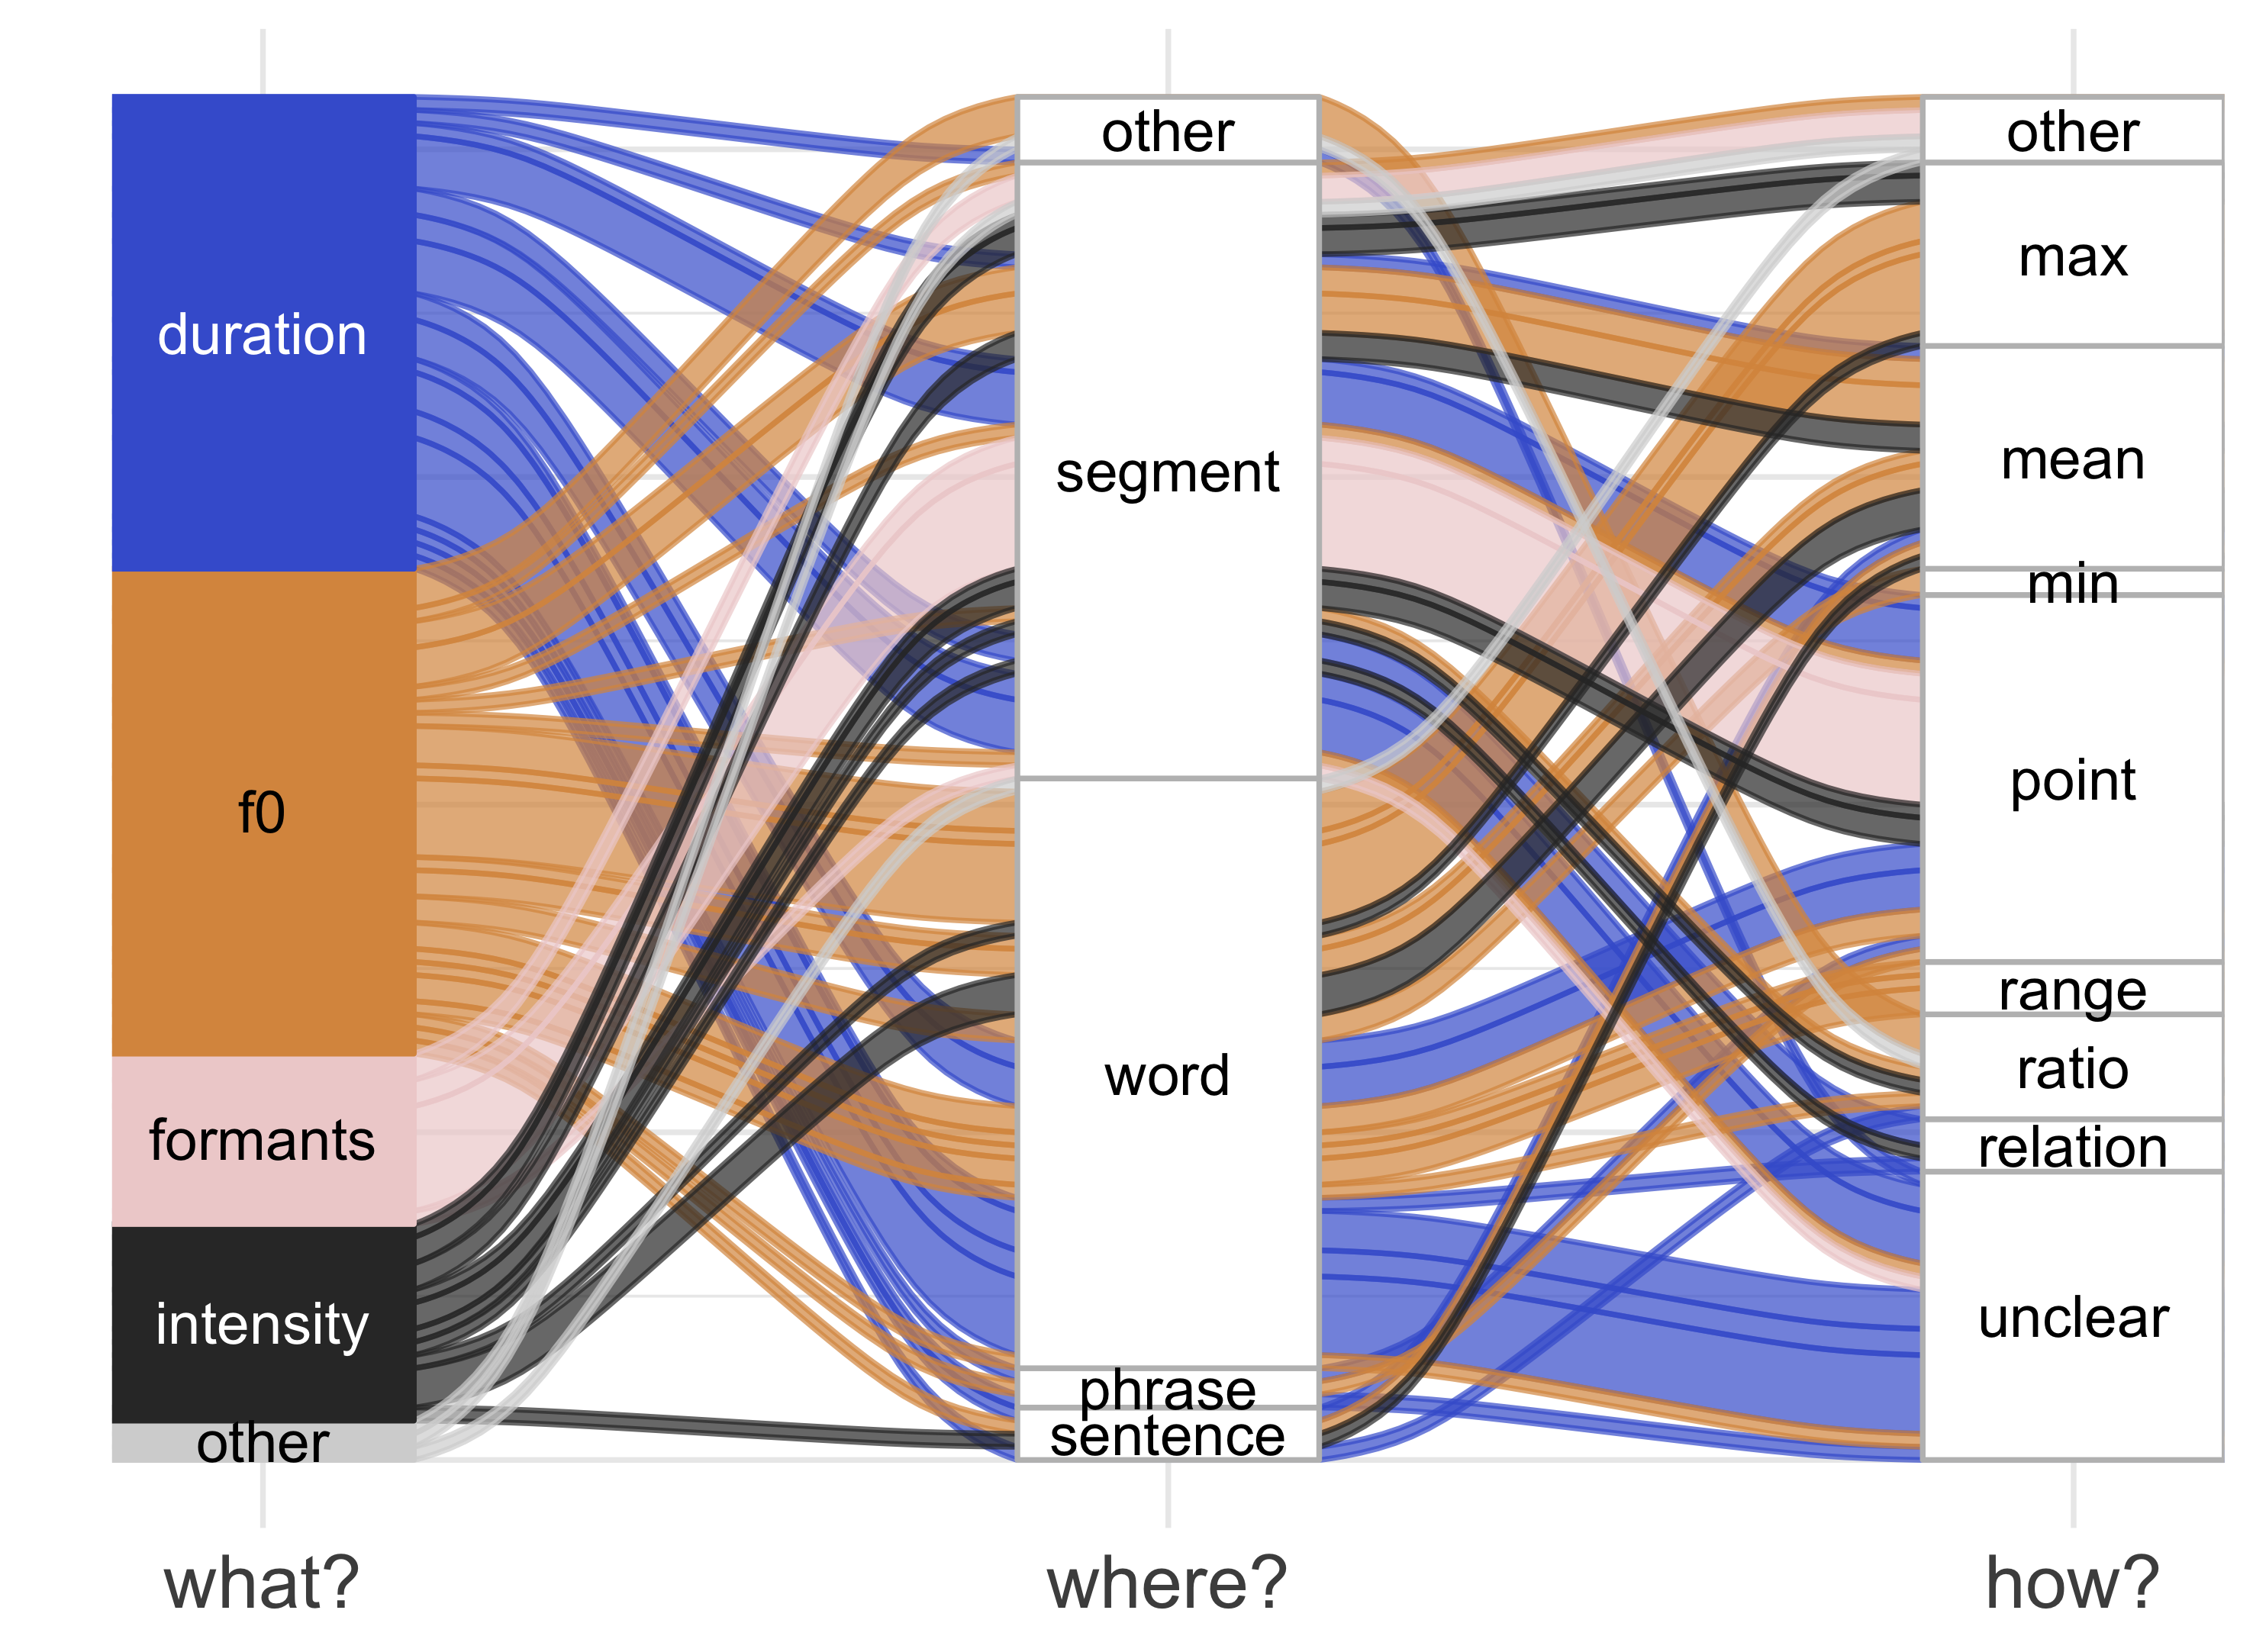
\includegraphics[width=1\linewidth]{./figs/flow_outcome} \caption{Sankey plot illustrating workflow choices from analyst teams.}\label{fig:sankey-plot}
\end{figure}

\begin{table}

\caption{\label{tab:descriptives-table}Descriptive statistics of all contributing teams and their acoustic and statistical analyses. The summary includes data from 46 teams and  159 analysts.}
\centering
\resizebox{\linewidth}{!}{
\fontsize{8}{10}\selectfont
\begin{tabular}[t]{llrr}
\toprule
\bf{Team characteristics} &    & \bf{Range} & \bf{Median}\\
\midrule
 & Team size & 1.0 -- 12.0 & 3.0\\
 & Years after PhD & -3.8 -- 16.0 & 4.7\\
 & Prior belief & 46.4 -- 92.8 & 70.0\\
 & Acoustic analysis peer rating & 36.5 -- 90.0 & 75.0\\
 & Statistical analysis peer rating & 22.5 -- 95.0 & 72.5\\
 & Overall peer rating & 20.0 -- 91.5 & 72.5\\
 &  &  \vphantom{5} & \\
\bf{Acoustic analyses} &  & \bf{n} & \bf{\%}\\
\midrule
\hspace{1em}Outcome & F0 & 51 & 35.9\\
 & Duration & 41 & 28.9\\
 & Intensity & 19 & 13.4\\
 & Formants & 18 & 12.7\\
 & Multivariate & 1 & 0.7\\
 & Other & 12 & 8.5\\
 &  &  \vphantom{4} & \\
\hspace{1em}Temporal window & Word & 60 & 42.9\\
 & Segment & 60 & 42.9\\
 & Phrase & 7 & 5.0\\
 & Sentence & 6 & 4.3\\
 & Pause & 1 & 0.7\\
 & Other & 6 & 4.3\\
 &  &  \vphantom{3} & \\
\hspace{1em}Typicality operationalization & Categorical & 95 & 69.3\\
 & Continuous (mean) & 33 & 24.1\\
 & Ordinal & 5 & 3.6\\
 & Continuous (median) & 3 & 2.2\\
 & Other & 1 & 0.7\\
 &  &  \vphantom{2} & \\
\bf{Statistical analyses} &  & \bf{n} & \bf{\%}\\
\midrule
\hspace{1em}Framework & Frequentist & 108 & 76.1\\
 & Bayesian & 27 & 19.0\\
 & Other & 7 & 4.9\\
 &  &  \vphantom{1} & \\
\hspace{1em}Model & Linear model & 125 & 88.0\\
 & GAM & 12 & 8.5\\
 & Machine learning & 3 & 2.1\\
 & Other & 2 & 1.4\\
 &  &  & \\
 &  & \bf{Range} & \bf{Median}\\
\hspace{1em}N & Models & 1 -- 16 & 2\\
 & Predictors & 1 -- 7 & 2\\
 & Random terms & 1 -- 10 & 2\\
\hspace{1em} & \hspace{1em}Intercept & \hspace{1em}1 -- 10 & \hspace{1em}2\\
\hspace{1em} & \hspace{1em}Slope & \hspace{1em}0 -- 5 & \hspace{1em}0\\
\bottomrule
\end{tabular}}
\end{table}

\end{document}
